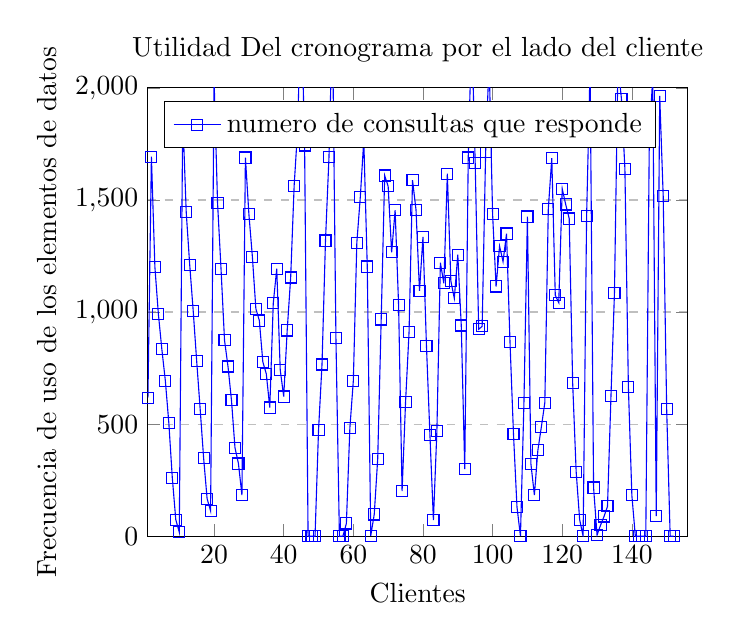
\begin{tikzpicture}
\begin{axis}[
    title={Utilidad Del cronograma por el lado del cliente},
    xlabel={Clientes},
    ylabel={Frecuencia de uso de los elementos de datos},
    xmin=1, xmax=156,
    ymin=0, ymax=2000,
    xtick={},
    ytick={},
    legend pos=north west,
    ymajorgrids=true,
    grid style=dashed,
]

\addplot[
    color=blue,
    mark=square,
    ]
    coordinates {
    %USO EXACTO
    (1,618)
(2,1693)
(3,1201)
(4,991)
(5,834)
(6,694)
(7,506)
(8,261)
(9,74)
(10,18)
(11,1873)
(12,1445)
(13,1211)
(14,1006)
(15,782)
(16,568)
(17,348)
(18,167)
(19,113)
(20,2035)
(21,1486)
(22,1191)
(23,874)
(24,757)
(25,606)
(26,395)
(27,324)
(28,183)
(29,1689)
(30,1437)
(31,1247)
(32,1015)
(33,962)
(34,778)
(35,724)
(36,574)
(37,1039)
(38,1193)
(39,742)
(40,623)
(41,918)
(42,1154)
(43,1564)
(44,1815)
(45,2413)
(46,1743)
(47,0)
(48,0)
(49,0)
(50,472)
(51,766)
(52,1319)
(53,1690)
(54,2298)
(55,884)
(56,0)
(57,0)
(58,57)
(59,482)
(60,694)
(61,1309)
(62,1513)
(63,1767)
(64,1203)
(65,2)
(66,97)
(67,345)
(68,967)
(69,1609)
(70,1561)
(71,1266)
(72,1454)
(73,1031)
(74,201)
(75,599)
(76,910)
(77,1588)
(78,1456)
(79,1094)
(80,1335)
(81,850)
(82,451)
(83,72)
(84,471)
(85,1220)
(86,1128)
(87,1617)
(88,1139)
(89,1061)
(90,1256)
(91,940)
(92,299)
(93,1689)
(94,2263)
(95,1664)
(96,923)
(97,936)
(98,1715)
(99,2119)
(100,1436)
(101,1114)
(102,1294)
(103,1225)
(104,1350)
(105,865)
(106,455)
(107,131)
(108,0)
(109,596)
(110,1426)
(111,323)
(112,183)
(113,383)
(114,487)
(115,596)
(116,1460)
(117,1686)
(118,1075)
(119,1042)
(120,1550)
(121,1480)
(122,1417)
(123,682)
(124,288)
(125,74)
(126,0)
(127,1427)
(128,2092)
(129,217)
(130,5)
(131,49)
(132,88)
(133,133)
(134,626)
(135,1086)
(136,2106)
(137,1952)
(138,1639)
(139,665)
(140,182)
(141,0)
(142,0)
(143,0)
(144,0)
(145,1761)
(146,2054)
(147,90)
(148,1964)
(149,1517)
(150,566)
(151,0)
(152,0)
    };
    \legend{numero de consultas que responde}

\end{axis}
\end{tikzpicture}

